%% LaTeX-Beamer template for KIT design
%% by Erik Burger, Christian Hammer
%% title picture by Klaus Krogmann
%%
%% version 2.1
%%
%% mostly compatible to KIT corporate design v2.0
%% http://intranet.kit.edu/gestaltungsrichtlinien.php
%%
%% Problems, bugs and comments to
%% burger@kit.edu

\documentclass[18pt]{beamer}
\usepackage[utf8x]{inputenc}
\usepackage{units}
\usepackage{booktabs}

%% CUSTOM
\usepackage{amsmath}
\usepackage{algpseudocode}

%% Definitions
\DeclareMathOperator{\div2}{div}
\renewcommand{\algorithmicrequire}{\textbf{Input:}}
\renewcommand{\algorithmicensure}{\textbf{Output:}}
\algnewcommand\algorithmicto{\textbf{to}}
\algrenewtext{For}[3]{\algorithmicfor\ $#1 \gets #2$ \algorithmicto\ $#3$ \algorithmicdo}
\algnewcommand\algorithmicod{\textbf{od}}
\algrenewtext{EndWhile}{\algorithmicod}
\algrenewtext{EndFor}{\algorithmicod}
%\AtBeginSection[]{%
%\begin{frame}<beamer> % do nothing in handouts
%    \frametitle{Überblick}
%    \tableofcontents[sectionstyle=show/shaded,
%    subsectionstyle=show/show/hide]
%\end{frame}
%}
%\AtBeginSubsection[]{%
%\begin{frame}<beamer> % do nothing in handouts
%    \frametitle{Überblick}
%    \tableofcontents[sectionstyle=show/shaded,
%    subsectionstyle=show/shaded/hide]
%\end{frame}
%}

%% SLIDE FORMAT

% use 'beamerthemekit' for standard 4:3 ratio
% for widescreen slides (16:9), use 'beamerthemekitwide'

\usepackage{templates/beamerthemekit}
%\usepackage{templates/beamerthemekitwide}

 %% TITLE PICTURE

 % if a custom picture is to be used on the title page, copy it into the 'logos'
 % directory, in the line below, replace 'mypicture' with the 
 % filename (without extension) and uncomment the following line
 % (picture proportions: 63 : 20 for standard, 169 : 40 for wide
 % *.eps format if you use latex+dvips+ps2pdf, 
 % *.jpg/*.png/*.pdf if you use pdflatex)


 \titleimage{banner}
 
 
%% Define some colors:
\definecolor{darkblue}{rgb}{0,0,.5}
\definecolor{darkgreen}{rgb}{0,.5,0}

 %% TITLE LOGO

 % for a custom logo on the front page, copy your file into the 'logos'
 % directory, insert the filename in the line below and uncomment it

\titlelogo{logo_150x150}
 
 % (*.eps format if you use latex+dvips+ps2pdf,
 % *.jpg/*.png/*.pdf if you use pdflatex)
 
 %% TikZ INTEGRATION
 
 % use these packages for PCM symbols and UML classes
 % \usepackage{templates/tikzkit}
 % \usepackage{templates/tikzuml}
 
 % the presentation starts here
 
\author{Dominik Muth - dominik.muth@student.kit.edu}
\institute{Institut f\"ur Informatik}


\title[Tutorium 3]{GBI Tutorium Nr. 32}
\subtitle{Tutorium 3}
\date{7. November 2012}

% Bibliography



\begin{document}

	%title page
	\begin{frame}
		\titlepage
	\end{frame}

	%table of contents
	\begin{frame}{Outline/Gliederung}
		\tableofcontents
	\end{frame}
	
	
	\section{\"Ubungsblatt 2}
	\begin{frame} {Übungsblatt 2}
		\begin{block} {Aufgabe 2.3}
			Gegeben ist folgende Aussage: \\
			\vspace{5pt}
			\hspace{10pt}$\bullet$ Jeder Mensch hat genau einen besten Freund.\\
			\vspace{5pt}
			Formalisieren Sie diese Aussage mit Hilfe des Prädikates $B(x,y)$ in Prädikatenlogik:\\
			$B(x,y)\mathrel{\widehat{=}} y$ ist bester Freund von $x$.
		\end{block}
		\begin{overprint}
			$M$ sei die Menge aller Menschen.
			\onslide<2> $\forall x \in M: \exists_1 y\in M:B(x,y)$ ?
			\onslide<3-> \color{red} $\forall x \in M: \exists_1 y\in M:B(x,y)$!\\
			
		\end{overprint}
		\begin{overprint}
			\onslide<4> $\forall x \in M: \exists y \in M: B(x,y)$
			\onslide<5> $\forall x \in M: \exists y \in M: B(x,y)\land \forall z \in  M \! \setminus \! y: \lnot B(x,z)$
			\onslide<6> \color{darkgreen}$\forall x \in M: \exists y \in M: B(x,y)\land \forall z \in  M \! \setminus \! y: \lnot B(x,z)$
		\end{overprint}
	
	\end{frame}	
		
	
	\section{Wiederholung} 
	\begin{frame} {Wiederholung}
		\begin{itemize}
			\item $M\cup \{\} =$ \only<1>{?} \only<2-> {\color{darkgreen}$M$}\\
			\color{black}
			\item $M\cap \{\} =$ \only<1-2>{?} \only<3-> {\color{darkgreen}$\{\}$}\\
			\color{black}
			\item $\{1,2,3\}\cup\{3,4,5\} =$ \only<1-3>{?} \only<4->{\color{darkgreen}$\{1,2,3,4,5\}$}\\
			\color{black}
			\item $\{1,2,3\}\setminus\{3,4,5\} =$ \only<1-4>{?} \only<5->{\color{darkgreen}$\{1,2\}$}\\
			\color{black}
			\item $((\{1,2,3\}\cup\{2,a,b\})\cap\{1,2,a,b,?\})\setminus \{1,a\}=$ \only<1-5>{?} \only<6->{\color{darkgreen}$\{2,b\}$}\\
		\end{itemize}
	\end{frame}
	
	
	\section{Formale Sprachen}
	\subsection{Definition}
	\begin{frame} {Formale Sprachen}
		\begin{block}{ Definition: formale Sprachen}
			Eine \textit{formale} Sprache (über dem Alphabet A), ist eine Teilmenge von $A^*$. Diese Sprache kann leer, endlich oder unendlich gro\ss{} sein.\\
			\vspace{5pt}
			Formal: $L\subset A^*$.
		\end{block}
		\begin{alertblock}{Achtung}
			$abb =$ Wort\\
			$\{abb\} =$ Sprache die das Wort \textit{abb} enthällt\\
			\vspace{5pt}
			$\Rightarrow abb \not= \{abb\}$ aber $abb \in \{abb\}$
		\end{alertblock}
	\end{frame}
	
	
	\subsection{Erklärung}
	\begin{frame} {Erklärung}
		\begin{block}{}
			L ist also eine Menge.\\
			L enthält alle syntaktisch korrekte Konkatenationen von Zeichen aus einem Alphabet A.
		\end{block}
	\end{frame}
	
	
	\subsection{Beispiele}
	\begin{frame}{Beispiel 1}
		\begin{exampleblock}{Schlüsselwörter in Java}
			Eine formale Sprache wäre zum Beispiel die Menge der Schlüsselwörter in der Programmiersprache Java:\\
			\vspace{5pt}
			\visible<2->{$\{\color{darkblue}int, double, if, else, for, while, \dots\color{black}\}$}\\
			\vspace{5pt}
			Grö\ss{}e: \visible<3>{endlich}
		\end{exampleblock}
	\end{frame}
	
	
	\begin{frame} {Beispiel 2}
		\begin{exampleblock}{Wörter ohne ''ab"}
			Gesucht ist eine Sprache $L$ aller Wörter über $A = \{\color{darkblue}a,b\color{black}\}$, in denen nirgends das Teilwort \color{darkblue}ab \color{black} vorkommt.\\
			\vspace{5pt}
			
			Formal: \visible<2->{
			$L=\{A^*\! \setminus \! \{ \omega_1 \color{darkblue}ab \: \color{black} \omega_2 \; | \; \omega_1,\omega_2 \in A^* \}$\\}
			\vspace{5pt}
			
			Alternativ: \visible<3-> {
			$L=\{ \omega_1 \omega_2 \; | \; \omega_1 \in \{\color{darkblue}b \color{black}\}^* \land\omega_2 \in \{\color{darkblue}a \color{black}\}^*$}\\
			\vspace{5pt}
			
			Grö\ss{}e: \visible<4> {unendlich}
		\end{exampleblock}
	\end{frame}
	
	
	\begin{frame} {Beispiel 3}
		\begin{exampleblock}{Ganze Zahlen $\mathbb{Z}$}
			\begin{itemize}
				\item Das Alphabet ist $A =$ 
				\visible<2->
				{$\{\color{darkblue}0,1,2,3,4,5,6,7,8,9,-\color{black}\}$}
				\pause
				\item Definition der Sprache L: 
				\visible<3->
				{$L= \{ \omega_1 \omega_2 \; | \; \omega_1 \in \{\epsilon, -\} \land \omega_2 \in (A \! \setminus \! \{-\})^+$}
				\pause
				\item $\Rightarrow -22 \in L$
				\pause
				\item $\Rightarrow 22-0- \not\in L$ $(aber \in A^*)$
				
			\end{itemize}
		\end{exampleblock}
	\end{frame}
	
	
	\subsection{Produkt / Konkatenation}
	\begin{frame} {Produkt / Konkatenation}
		\begin{block}{Definition: Produkt}
			Wie bei Wörtern, lassen sich auch formale Sprachen Konkatenieren:\\
			Sei $L_1$ und $L_2$ zwei formale Sprachen. Dann bezeichnet\\
			\vspace{5pt}
			\hspace{10pt}			
			$L_1 \cdot L_2 = \{\omega_1 \omega_2 \; | \; \omega_1 \in L_1 \land \omega_2 \in L_2\}$\\
			\vspace{5pt}
			Das Produkt, bzw. die Konkatenation der Sprachen $L_!$ und $L_2$.
		\end{block}
		
		\pause		
		
		\begin{exampleblock}{Beispiel: Wörter ohne ''ab"}
			Statt $L=\{ \omega_1 \omega_2 \; | \; \omega_1 \in \{\color{darkblue}b \color{black}\}^* \land\omega_2 \in \{\color{darkblue}a \color{black}\}^*$ \\
			Lässt sich die Sprache schreiben als: 
			\visible<2>{$L = \{a\}^*\{b\}^*$}
		\end{exampleblock}
	\end{frame}


	\begin{frame}{Aufgaben}
		\begin{block} {Aufgabe 1}
			Gegeben seien die Sprache $L_1$ mit $L_1 = \{a^n\; | \; n \in \mathbb{N}_0 \}$\\
			und $L_2$ mit $L_2 = \{b^n \; | \; n \in \mathbb{N}_0 \}$\\
			Sind folgende Wörter $\in L_1 \cdot L_2$?
			\begin{itemize}
				\item ab 
				\visible<2-> {\color{darkgreen}$\surd$ \color{black}}
				\item $\epsilon$
				\visible<3-> {\color{darkgreen}$\surd$ \color{black}}
				\item bab
				\visible<4-> {\color{red}$X$ \color{black}}
				\item aaaaa
				\visible<5-> {\color{darkgreen}$\surd$ \color{black}}
			\end{itemize}
		\end{block}
		\pause
		\pause
		\pause
		\pause
		\pause
		\begin{alertblock}{Achtung}
			$L_1L_2 \not = \{a^n b^n \; | \; n \in \mathbb{N}\}$\\
			da die Exponenten verschieden sein können gilt:\\
			$L_1L_2 = \{a^n b^m \; | \; n,m \in \mathbb{N}\}$
		\end{alertblock}
	\end{frame}


	\subsection{Potenzen}
	\begin{frame}{Potenzen}
		\begin{block}{Definition: Potenzen}
			Ebenso wie bei Alphabeten und Wörtern lassen sich auch bei Sprachen Potenzen bilden.\\
			Sei $L$ eine formale Sprache mit: $L = \{the, cake, is, a, lie\}$\\
			Dann gilt:\\
			\begin{itemize}
				\item \visible<2->{$L^0 = \{\epsilon\}$}
				\item \visible<3->{$L^1 = L$}
				\item \visible<4->{$L^2 = L \cdot L = \{thecake, theis, thea, thelie, \dots\}$}
				\item \visible<5->{$\Rightarrow L^{i+1} = L^i \cdot L$
				 (rekursive Definition)}
				\item \visible<6->{In was liegt: "the cake is a lie"?}\\
				\visible<7-> {\color{red} \hspace{10pt}
				In nichts, da das Leerzeichen: 
				$(\textvisiblespace)$ gänzlich in der Sprache $L$ fehlt.}
			\end{itemize}
		\end{block}
	\end{frame}
	
	
	\subsection{Konkatenationsabschluss}
	\begin{frame}{Konkatenationsabschluss}
		\begin{block}{Definition: Konkatenationsabschluss}
			Sei L eine formale Sprache, dann ist der Konkatenationsabschluss:
			\begin{displaymath}
				L^* = \bigcup_{i=0}^{\infty}L^i
			\end{displaymath}
			\pause
			Der $\epsilon$-freie Konkatenationsabschluss sei dann definiert durch:
			\begin{displaymath}
				L^+ = \bigcup_{i=1}^{\infty}L^i
			\end{displaymath}
		\end{block}
	\end{frame}


	\begin{frame}{Konkatenationsabschluss}
		\begin{alertblock}{$\epsilon$-freier Konkatenationsabschluss}
			In der Regel gilt zwar: $\epsilon \not\in L^+$,\\
			Wenn allerdings gilt: $\epsilon \in L \Rightarrow \epsilon \in L^+$
		\end{alertblock}
	\end{frame}
	
	
	\section{Aufgaben}
	\begin{frame} {Aufgaben}
		\begin{block} {easy going}
			$L$ soll alle Wörter enthalten, welche genau ein $b$ enthalten.\\
			Gegeben sei dazu das Alphabet: $A = \{a,b\}$\\
			\vspace{10pt}
			\visible<2> {
				\begin{itemize}
					\item $L = \{a\}^* \cdot \{b\} \cdot \{a\}^*$
					\item $L = \{\omega_1b\omega_2 \; | \; \omega_1, \omega_2 \in \{a\}^*\}$
				\end{itemize}
			}
		\end{block}
	\end{frame}

		
	\begin{frame} {Aufgaben}
		\begin{block} {possible to do}
			Es sei $A = \{a,b\}$. Beschreiben Sie die folgenden formalen Sprachen mit den Symbolen $\{$, $\}$, $a$, $b$, $*$, $\epsilon$, Komma, $($, $)$ und +:
			\begin{itemize}
				\item die Menge aller Wörter über A, die das Teilwort ''ab'' enthalten.\\
				\visible<2->{\color{darkgreen}
					$L = \{a,b\}^*\{ab\}\{a,b\}^*$
				\color{black}}
				\item die Menge aller Wörter über A, deren vorletztes Zeichen ein "b'' ist.\\
				\visible<3->{\color{darkgreen}
					$L = \{a,b\}^*\{b\}\{a,b\}$
				\color{black}}
				\item die Menge aller Wörter über A, in denen nirgends zwei "b''s hintereinander vorkommen.\\
				\visible<4->{\color{darkgreen}
					$L = \{a, ba\}^*\{b, \epsilon\}$
				\color{black}}
			\end{itemize}
		\end{block}
	\end{frame}

		
	\begin{frame} {Aufgaben}
		\begin{block} {badass}
			Gegeben seien die Formalen Sprachen $L_1$ und $L_2$:\\
			\hspace{10pt}
			$L_1=\{a^kb^m \; | \; k,m\in\mathbb{N}_0 \land k \; mod \; 2 = 0 \land m \; mod \; 3 = 1\}$\\
			\hspace{10pt}
			$L_2=\{b^ka^m \; | \; k,m\in\mathbb{N}_0 \land k \; mod \; 2 = 1 \land m \; mod \; 3 = 0\}$\\
			Drücken sie folgende Sprachen in Mengenschreibweise aus:
			\begin{itemize}
				\item $L = L_1$\\
				\visible<2->{\color{darkgreen}
					$L = \{aa\}^*\{b\}\{bbb\}^*$
				\color{black}}
				\item $L = L_1 \cdot L_2$\\
				\visible<3->{\color{darkgreen}
					$L = \{aa\}^*\{b\}\{bbb\}^*\{b\}\{bb\}^*\{aaa\}^*$
				\color{black}}
				\item $L = L_1 \cap L_2$\\
				\visible<4->{\color{darkgreen}
					$L = \{b\}\{bbbbbb\}^*$
				\color{black}}
			\end{itemize}
		\end{block}
	\end{frame}
	
	
	
	
	\section{Fragen}
	\begin{frame} {Fragen}
		\begin{itemize}
			\item Fragen zum Stoff?
			\item Fragen zum n\"achsten \"Ubungsblatt?
			\item Generelle Fragen?
		\end{itemize}
	\end{frame}
	
	
	\begin{frame} {EOF}
		\begin{center}
			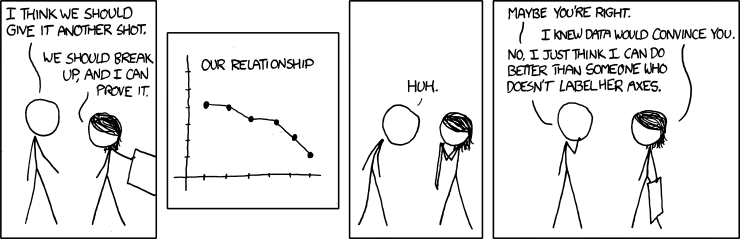
\includegraphics[scale=0.45]{graphics/eof3.png}\\
			\tiny $source: imgs.xkcd.com/comics/convincing.png$
		\end{center}
	\end{frame}

\end{document}
